\documentclass[11pt]{article}
\usepackage{subfigure,wrapfig,graphicx,booktabs,fancyhdr,amsmath,amsfonts}
\usepackage{bm,amssymb,amsmath,amsthm,wasysym,color,fullpage,setspace,multirow}
\usepackage{listings, xcolor}
\usepackage{pdfpages}
\usepackage{siunitx}
\newcommand{\vb}{\boldsymbol}
\newcommand{\vbh}[1]{\hat{\boldsymbol{#1}}}
\newcommand{\vbb}[1]{\bar{\boldsymbol{#1}}}
\newcommand{\vbt}[1]{\tilde{\boldsymbol{#1}}}
\newcommand{\vbs}[1]{{\boldsymbol{#1}}^*}
\newcommand{\vbd}[1]{\dot{{\boldsymbol{#1}}}}
\newcommand{\vbdd}[1]{\ddot{{\boldsymbol{#1}}}}
\newcommand{\by}{\times}
\newcommand{\tr}{{\rm tr}}
\newcommand{\cpe}[1]{\left[{#1} \times \right]}
\newcommand{\sfrac}[2]{\textstyle \frac{#1}{#2}}
\newcommand{\ba}{\begin{array}}
\newcommand{\ea}{\end{array}}
\renewcommand{\earth}{\oplus}
\newcommand{\sinc}{{\rm \hspace{0.5mm} sinc}}
\newcommand{\tf}{\tilde{f}}
\newcommand{\tbox}[1]{\noindent \fbox{\parbox{\textwidth}{#1}}}
\DeclareMathAlphabet{\mathpzc}{OT1}{pzc}{m}{it}
\definecolor{mylilas}{RGB}{170,55,241}
\definecolor{mygreen}{RGB}{0,168,45}


\title{ASE 389P.4 Methods of Orbit Determination \\ Final Project Submission}
\author{Corey L Marcus} \date{Wednesday, May 12\textsuperscript{th}}

%command to write C++ nicely
\def\CC{{C\nolinebreak[4]\hspace{-.05em}\raisebox{.4ex}{\tiny\bf ++}}}

%commands to include C++ code in appendix
\lstset { %
	language=C++,
	backgroundcolor=\color{black!5}, % set backgroundcolor
	basicstyle=\tiny,% basic font setting
}

\begin{document}
\onehalfspace
\maketitle

\abstract{ {\bf Redo this }This phase of the project shows the initial attempt at orbital determination. The estimation scheme involves a nonlinear least-squares based estimator initialization followed by a standard Unscented Kalman Filter.}

\section{Introduction}

This report documents the first stage of the final project. We are provided approximately 24 hours of satellite range and range-rate measurements from three ground based stations. Our objective is to use these measurements to deliver a satellite state estimate seven days after the initial epoch. \\

The following sections document the methodology used, including system dynamics modeled, approximations made, and estimation schemes used. Then deliverables are displayed and discussed. Finally, estimator performance is evaluated.

\section{Methodology}

\subsection{System Dynamics}

This subsection details the system dynamics used to model the spacecraft's orbit. All code was written in {\CC} for its increased speed when compared to scripting languages such as MATLAB. Many of the algorithms used were sourced from the well-known text "\textit{Fundamentals of Astrodynamics and Applications}" by David Vallado.

\subsubsection{Gravity Model}

An EGM-96 gravity model was used up to a 20x20 gravity field. The choice to use {\CC} was motivated primarily by the computational expense of this gravity model. A slower language such as MATLAB would have much longer propagation times for the same complexity gravity model.

\subsubsection{Drag Model}

A simple cannonball drag model was used due to the relatively small effect of drag on the spacecraft's orbit. The cross-sectional area of the spacecraft was approximated at \SI{22}{\meter\squared} and the coefficient of drag at 1.88.

\subsubsection{Solar Radiation Pressure Model}

Similar to atmospheric drag, a simple cannonball model was used to model Solar Radiation Pressure (SRP). SRP force is not modeled when the spacecraft is shielded from the sun by the Earth's shadow. The coefficient of drag for SRP was approximated as 0.1. It was noted that the system had a very low sensitivity to SRP so limited effort was applied to its estimation and modeling.

\subsubsection{Luni-Solar Model}

Third body gravitational effects from the Sun and Moon were included. The acceleration due to each of these bodies was found according to a simple point-mass gravitational model. This simplification is justified due to the significant distance between the spacecraft and each of the third bodies. Algorithms to locate the Sun and Moon as a function of the current UTC time were found in \textit{Vallado}.

\subsection{Measurement Model}

A standard range and range-rate measurement model were used to generate predicted measurements. One difficulty is that the speed of light must be accounted for in determining when to utilize a measurement. Noting that the signal to noise ratio of the range measurements is extremely high, the measurement was used directly along with the speed of light in determining its time of flight. The measurement update was therefore applied at the time of receipt minus the time of flight.

\subsection{Estimation}

The estimation scheme centers around an Unscented Kalman Filter (UKF). The UKF is a nonlinear extension of the standard Kalman Filter. Its hallmark is approximation of covariances in the propagation and update phase through numerical propagation of a collection of sigma points chosen to conveniently represent the distribution of the prior. After propagation through time or into the measurement space, approximations of the mean and variance of the transformed distribution can be found by investigating the spacial distribution of the sigma points. It was chosen over the more traditional Extended Kalman Filter (EKF) because it does not require explicit computation of the state-transition matrix. The true STM in this case is complex mathematically and computationally. Approximations of the STM would not serve us well over the long intervals without measurements. \\

A ``$2n+1$" number of points were used along with a single tuning parameter $k=0.5$. This value was chosen so that all sigma points would be given the same weight. \\

The choice was made to estimate only position and velocity due to the limited quality of the dynamics model. If items such as coefficient of drag and sensor biases are to be estimated, a much higher quality model with lower process noise is needed due to rather weak observability of these quantities. \\

Filter initialization is a challenge for many nonlinear extensions of the Kalman Filter. Improper initialization can quickly lead to filter divergence. A nonlinear least-squares optimization scheme was used to find the initial state estimate. This involved using Levenberg-Marquardt (LM) to select the initial state, $x_0$, such that the norm of the prefit residuals, Equation \eqref{eq:ICcost}, was minimized. To reduce the computational complexity, only the first 50 measurements were considered. In Equation \eqref{eq:ICcost} $f_a^b(\cdot)$ represents the nonlinear propagation of the satellite's state from the time of measurement $a$ to $b$, $h(\cdot)$ represents the measurement dynamics, and $z_i$ represents the $i$\textsuperscript{th} measurement. 

\begin{equation}
	\label{eq:ICcost}
	J(x_0) = \sum_{i=0}^{i=50} \left( z_i - h(f_{0}^{i}(x_0)) \right)^2 
\end{equation}

The resulting $x0$ is shown in Equation \eqref{eq:LM_IC}. The units are $km$ and $km/s$. The initial estimate covariance, $P_0$, was chosen arbitrarily to achieve a filter which converged for all test cases. This matrix is shown in Equation \eqref{eq:P0}. To correspond with the state, the units are $km^2$ and $km^2/s^2$. $diag \{a, b, c, ... \}$ is shorthand for a diagonal matrix with its arguments on the diagonal.

\begin{equation}
	\label{eq:LM_IC}
	x_0 = \begin{bmatrix}
	6980.3967323588 \\
	1619.61802198332 \\
	15.1399428739289 \\
	-1.66690187359566 \\
	7.2578409459164 \\
	0.261907498000759 \\	
	\end{bmatrix}
\end{equation}

\begin{equation}
	\label{eq:P0}
	P_0 = diag \{ 100, 100, 100, 0.01, 0.01, 0.01 \}
\end{equation}

An attempt was made to use the LM optimizer to find estimates of the drag coefficient and sensor biases as well, but these did not prove fruitful. The sensitivity to sensor biases seems too low for the LM algorithm to detect. When attempting to optimize $C_d$, the system rapidly increases $C_d$ towards infinity for unknown reasons. Further investigation is needed in this area to improve estimator performance. \\

Process noise is an important component of estimation used to account for unmodeled dynamics and inputs to the system. The process noise covariance, $Q$, was modeled according to the suggestion in the Final Project Assignment and is shown in Equation \eqref{eq:Q}. The size of the component $\sigma^2$ was chosen manually to produce adequate filter performance. This value was found to be $\sigma^2 = 5$E$-15$.

\begin{equation}
\label{eq:Q}
Q = \Delta t^2 \begin{bmatrix}
\frac{\Delta t^2}{4} \sigma^2 & 0 & 0 & \frac{\Delta t}{2} \sigma^2 & 0 & 0 \\
0 & \frac{\Delta t^2}{4} \sigma^2 & 0 & 0 & \frac{\Delta t}{2} \sigma^2 & 0 \\
0 & 0 & \frac{\Delta t^2}{4} \sigma^2 & 0 & 0 & \frac{\Delta t}{2} \sigma^2 \\
\frac{\Delta t}{2} \sigma^2 & 0 & 0 & \sigma^2 & 0 & 0 \\
0 & \frac{\Delta t}{2} \sigma^2 & 0 & 0 & \sigma^2 & 0 \\
0 & 0 & \frac{\Delta t}{2} \sigma^2 & 0 & 0 & \sigma^2 \\	
\end{bmatrix}
\end{equation}

\section{Deliverables}

\subsection{Prefit Residuals}

Figure \ref{fig:prefit} shows the prefit measurement residuals when all measurement types and sensors are considered. To better demonstrate detail Figure \ref{fig:prefit_zoom} shows a zoomed-in plot of the measurement residuals.

\begin{figure}[!htb]
	\centering
	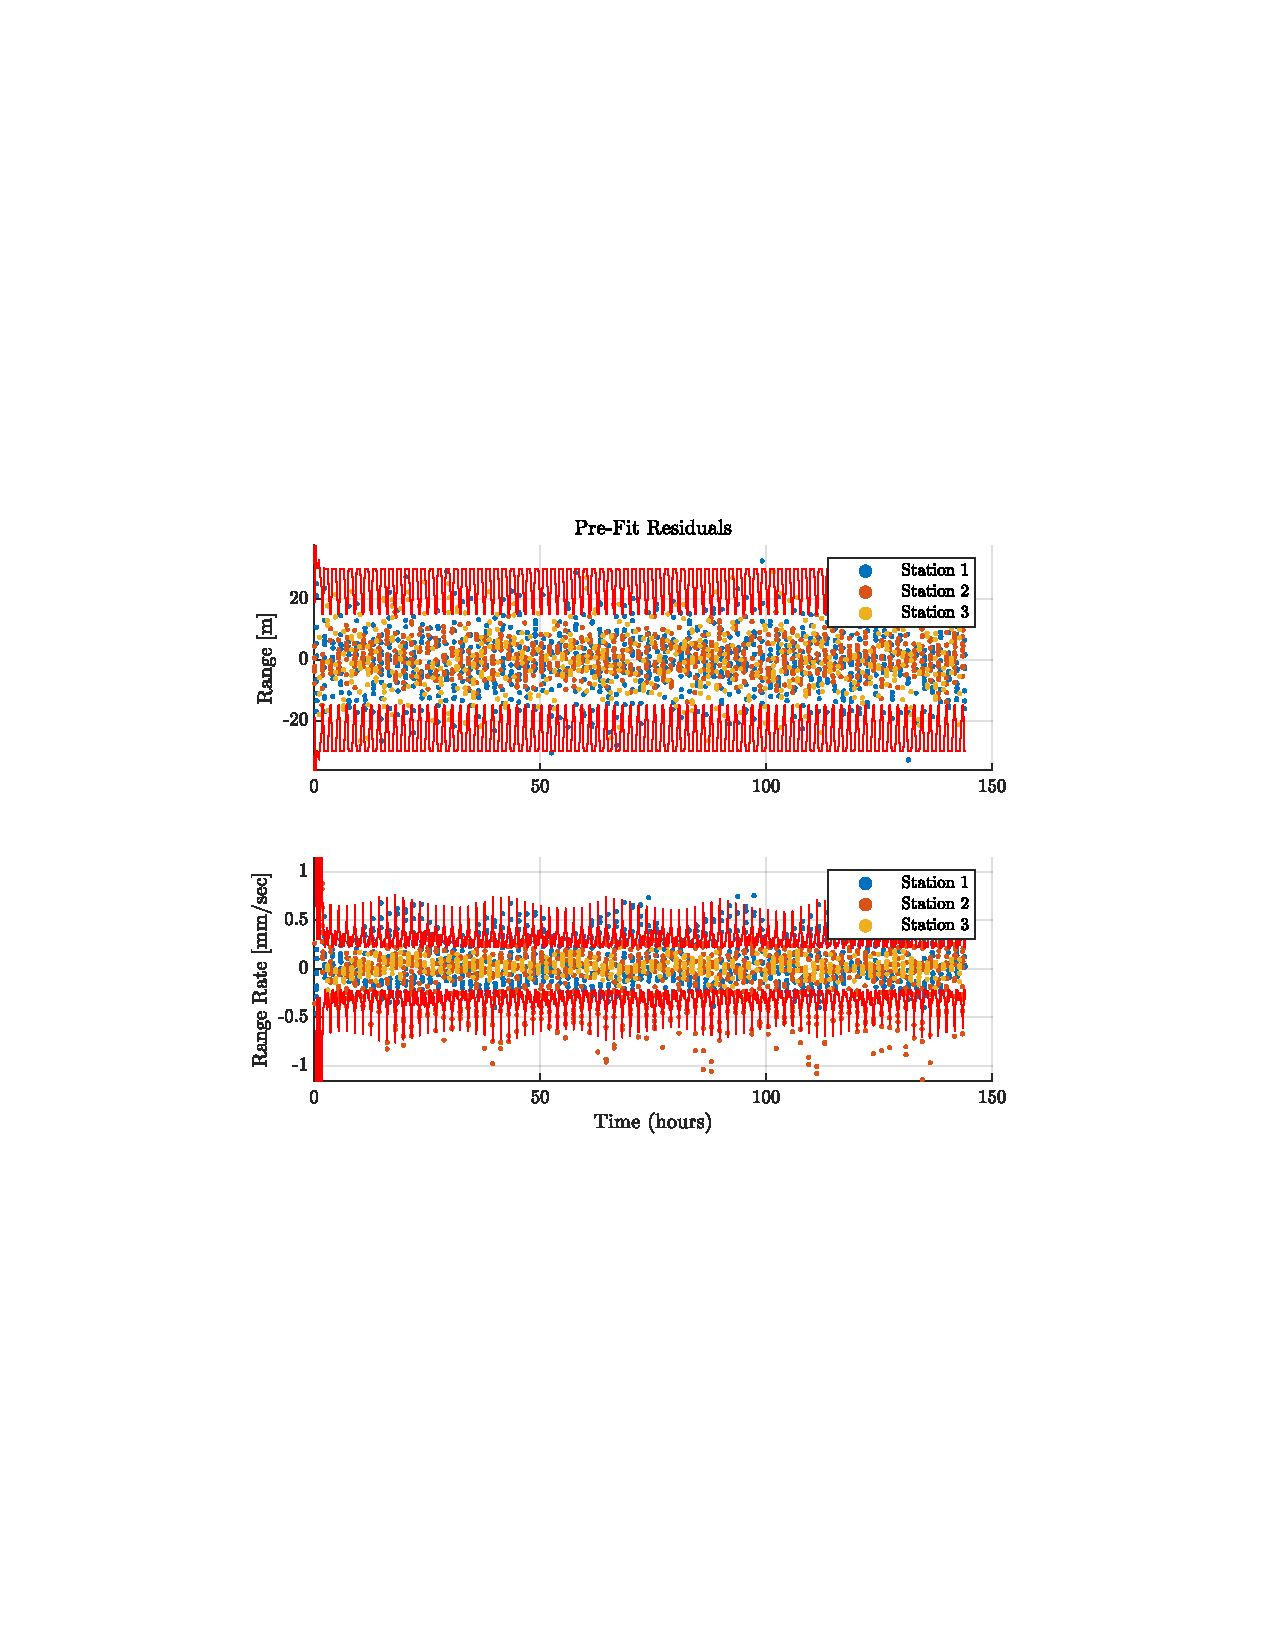
\includegraphics[clip,trim=4cm 8.5cm 4cm 8.5cm, width=.5\textwidth]{figs/prefit_res_final.pdf}
	\caption{The prefit measurement residuals for range (top) and range-rate (bottom).}
	\label{fig:prefit}
\end{figure}

\begin{figure}[!htb]
	\centering
	\includegraphics[width=.9\linewidth]{figs/prefitres_zoom.png}
	\caption{A zoomed for clarity view of the prefit measurement residuals for range (top) and range-rate (bottom).}
	\label{fig:prefit_zoom}
\end{figure}

\subsection{Postfit Residuals}

Figure \ref{fig:postfit} shows the postfit measurement residuals when all measurement types and sensors are considered. To better demonstrate detail Figure \ref{fig:postfit_zoom} shows a zoomed-in plot of the measurement residuals.

\begin{figure}[!htb]
	\centering
	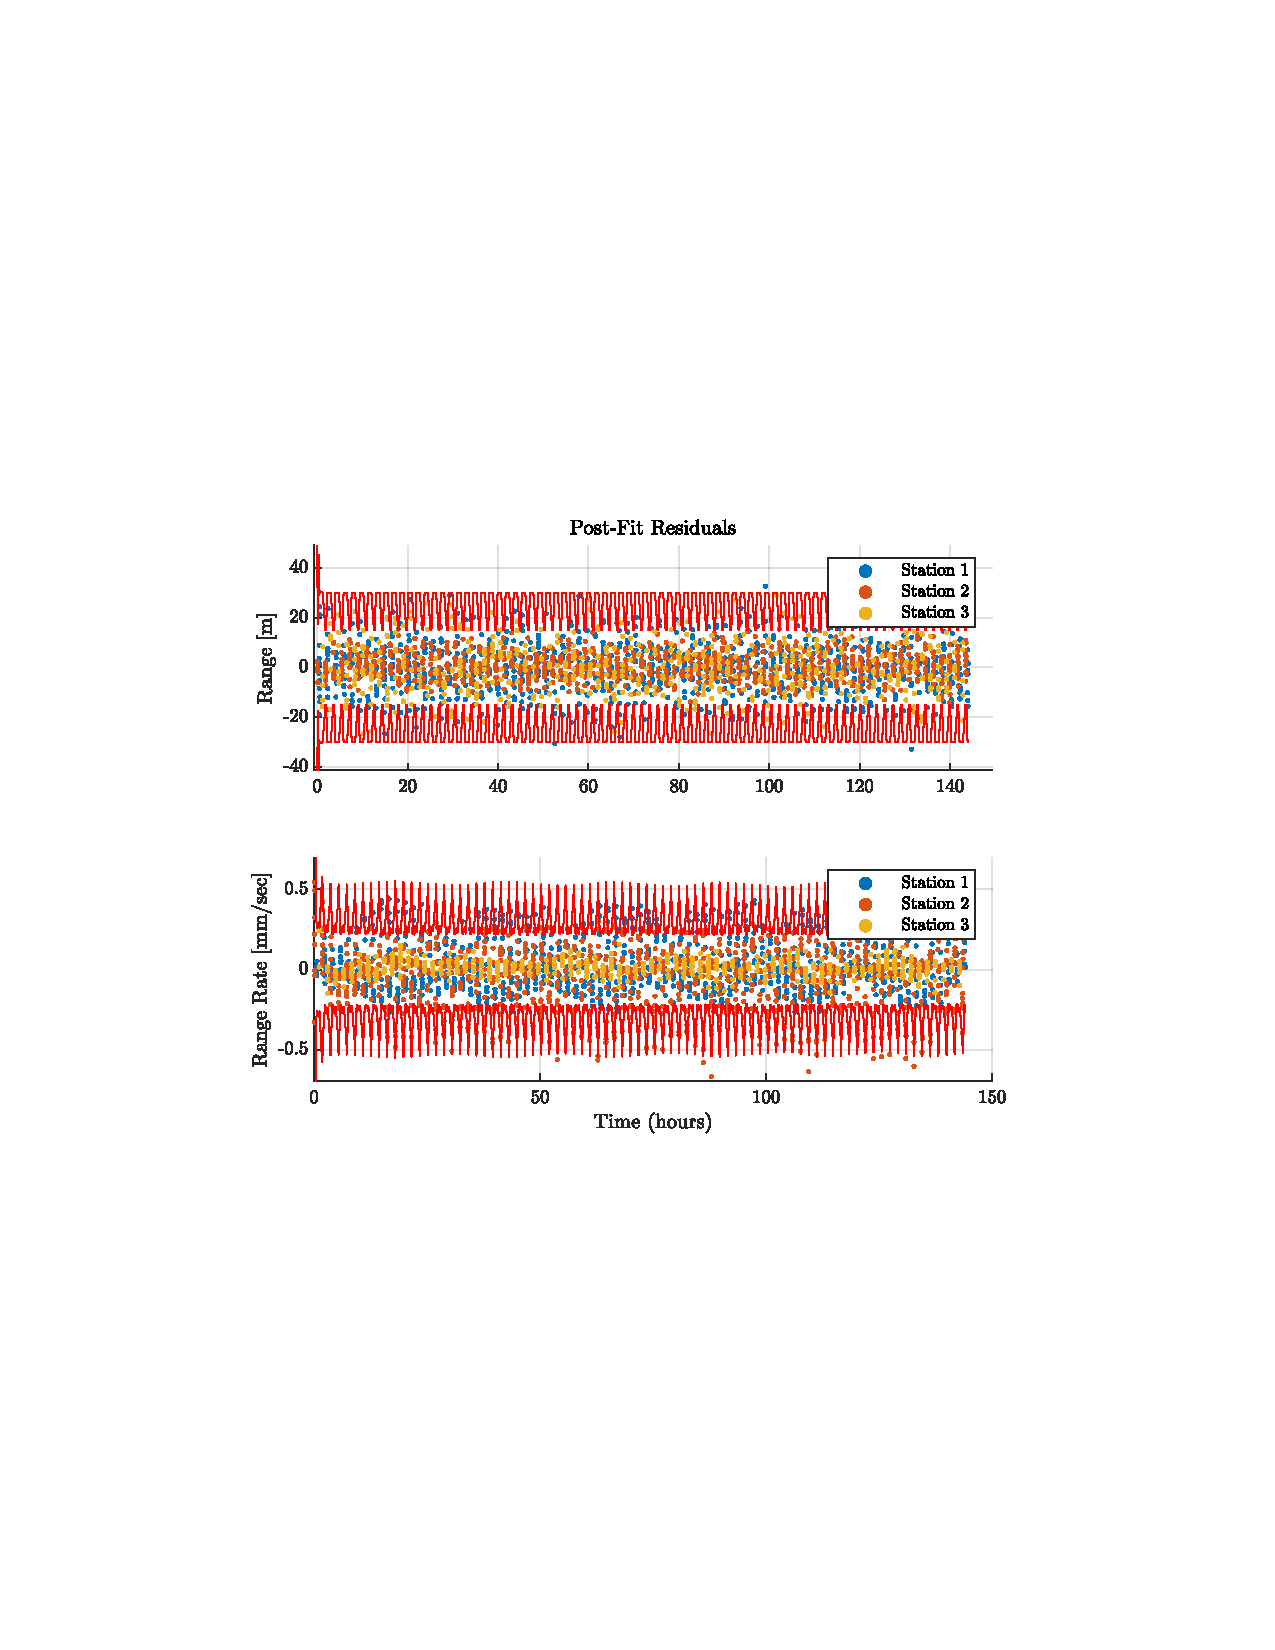
\includegraphics[clip,trim=4cm 8.5cm 4cm 8.5cm, width=.5\textwidth]{figs/postfit_res_final.pdf}
	\caption{The postfit measurement residuals for range (top) and range-rate (bottom).}
	\label{fig:postfit}
\end{figure}

\begin{figure}[!htb]
	\centering
	\includegraphics[width=.9\linewidth]{figs/postfitres_zoom.png}
	\caption{A zoomed for clarity view of the postfit measurement residuals for range (top) and range-rate (bottom).}
	\label{fig:postfit_zoom}
\end{figure}

\subsection{State Estimates at $\Delta V_1$}

To investigate the consistency of the estimates, case F (all data and all sensors) was designated as the best estimated trajectory. A transformation was found to map vectors into the Radial-Intrack-Crosstrack (RQW) coordinate frame described by the best estimate. For each case, the associated deviation from best-estimate and estimate covariance was transformed into the RQW frame. Figures \ref{fig:rad_cross}, \ref{fig:rad_in}, and \ref{fig:cross_in} showcase these deviations and covariances.

\begin{figure}[!htb]
	\centering
	\includegraphics[width=.9\linewidth]{figs/rad_cross.png}
	\caption{The $\Delta V_1$ state estimates for each case expressed in the RQW frame defined by the best estimate. Shown here is a 2D slice of the estimates in the radial and crosstrack directions.}
	\label{fig:rad_cross}
\end{figure}

\begin{figure}[!htb]
	\centering
	\includegraphics[width=.9\linewidth]{figs/rad_in.png}
	\caption{The $\Delta V_1$ state estimates for each case expressed in the RQW frame defined by the best estimate. Shown here is a 2D slice of the estimates in the radial and intrack directions.}
	\label{fig:rad_in}
\end{figure}

\begin{figure}[!htb]
	\centering
	\includegraphics[width=.9\linewidth]{figs/cross_in.png}
	\caption{The $\Delta V_1$ state estimates for each case expressed in the RQW frame defined by the best estimate. Shown here is a 2D slice of the estimates in the intrack and crosstrack directions.}
	\label{fig:cross_in}
\end{figure}

 
\section{Discussion}

From the Deliverables, we can form a variety of conclusions. We begin with a discussion of the prefit residuals. First we note that residuals at the beginning of the epoch are low, this indicates that our LM optimization scheme has most likely provided us an accurate initial state estimate. We also note that residuals are high immediately after a measurement gap; this is expected. Any estimation error immediately before a measurement gap is bound to grow during the nonlinear orbital propagation without any updates. Even if we had perfect estimation, error is bound to grow due to the unmodeled dynamics of our system. It is possible that our simplifications in dynamics modeling are contributing significantly to the growth of these residuals. We may be able to increase estimator performance by increasing the fidelity of our drag and SRP models. \\

These large residuals also indicate that our estimate propagation to $\Delta V_1$ is likely to contain significant error. Another area for concern is the fact that many residuals are outside of their $3\sigma$ bounds. This shows that the filter is not accurately representing its own performance and is over-confident. A likely source of this behavior is mismodeled process noise. The process noise is likely too low and does not accurately encompass the differences between the model and truth. Another potential source of error is measurement biases. As discussed before, the system dynamics do not seem accurate enough to estimate these biases, further iterations of the project will attempt to do so. \\

Next, we discuss the postfit residuals. Again, the residuals do not appear to change much in magnitude with time. This provides more evidence that the LM initial estimate is a relatively accurate one. There is clear structure in the postfit residuals for range measurements as they follow a roughly linear trend during each set of observations. This is not the expected performance for measurement residuals. Ideally, these postfit residuals should resemble white stochastic noise. The unmodeled structure can be accounted for to get better estimate performance at a later point in the project. Finally, a large number of the residuals exist outside of the $3\sigma$ boundaries. This all points to unmodeled system dynamics. \\

Finally, we discuss the plots of our estimates in the RQW coordinate system. This segment of the project involves a day's worth of measurements followed by six days of propagation. Even minute initial differences in state will result in large differences after six days of orbit propagation without measurement update. With this in mind, it is no surprise that the estimates differ wildly from each other. It is reasonable to assume that these estimates also differ strongly from the true satellite state, especially in light of previous discussions on unmodeled dynamics. One would expect the measurement covariances of the different estimates to align somewhat, in other words a well designed estimator would estimate its own uncertainty well. This is not the case for the estimates shown here. Almost none of the estimate covariances overlap. This provides additional evidence that the process noise of the system is not well accounted for. \\

With these inefficiencies in mind, it is difficult to draw conclusions on the relative performance of each case. However, one would expect cases with more measurements to perform better than those with fewer. Additionally, we expect measurements of range to provide more information than range-rate as position measurements can be analyzed in aggregate to provide estimates of velocity while the reverse can not be said to be true. \\

\section{Conclusion}

In conclusion, we have demonstrated a modest estimation scheme with plenty of room for improvement. While estimates of satellite state at the delivery time are provided, analysis of measurement residuals and the consistency of these estimates suggests their quality may be poor. \\

A number of areas for improvement have been identified. These include increasing drag and SRP model fidelity, better process noise tuning, and estimating secondary parameters such as coefficient of drag and measurement biases. The project reports following this one will attempt to address these problems to produce higher quality final estimates.


\newpage
\appendix
\section{Code}

\subsection{\texttt{main.cc}}
\lstinputlisting{../../src/project/main.cc}

%%plot matlab files now
%\lstset { %
%	language=matlab,
%	backgroundcolor=\color{black!5}, % set backgroundcolor
%	basicstyle=\tiny,% basic font setting
%}

\subsection{\texttt{VehicleState.h}}
\lstinputlisting{../../src/project/VehicleState.h}

\subsection{\texttt{Estimators.h}}
\lstinputlisting{../../src/project/Estimators.h}

\subsection{\texttt{Util.h}}
\lstinputlisting{../../src/project/Util.h}

\subsection{\texttt{VehicleState.cc}}
\lstinputlisting{../../src/project/VehicleState.cc}

\subsection{\texttt{Estimators.cc}}
\lstinputlisting{../../src/project/Estimators.cc}

\subsection{\texttt{Util.cc}}
\lstinputlisting{../../src/project/Util.cc}

\end{document}
